%-------------------------
% Resume in Latex
% Author : Amlaan Bhoi
% Adapted from: Sourabh Bajaj
% License : MIT
%------------------------

\documentclass[letterpaper,10pt]{article}

\usepackage{latexsym}
\usepackage[empty]{fullpage}
\usepackage{titlesec}
\usepackage{marvosym}
\usepackage[usenames,dvipsnames]{color}
\usepackage{verbatim}
\usepackage{enumitem}
\usepackage[pdftex, hidelinks]{hyperref}
\usepackage{fancyhdr}
\usepackage{pdfpages}

\usepackage[charter]{mathdesign} % Bitstream Charter
% \usepackage{newpxtext,newpxmath} % Palatino

\pagestyle{fancy}
\fancyhf{} % clear all header and footer fields
\fancyfoot{}
\renewcommand{\headrulewidth}{0pt}
\renewcommand{\footrulewidth}{0pt}

% Adjust margins
\addtolength{\oddsidemargin}{-0.50in}
\addtolength{\evensidemargin}{-0.50in}
\addtolength{\textwidth}{1in}
\addtolength{\topmargin}{-.5in}
\addtolength{\textheight}{1.0in}

\urlstyle{same}

\raggedbottom
\raggedright
\setlength{\tabcolsep}{0in}

% Sections formatting
\titleformat{\section}{
  \vspace{-6pt}\scshape\raggedright\large
}{}{0em}{}[\color{black}\titlerule \vspace{-5pt}]

%-------------------------
% Custom commands
\newcommand{\resumeItem}[2]{
  \item\small{
    \textbf{#1}{: #2 \vspace{-2pt}}
  }
}

\newcommand{\resumeItemNoBullet}[2]{
  \item[]\small{
    \hspace{-9pt}\textbf{#1}{: #2 \vspace{-6pt}}
  }
}

\newcommand{\resumeSubheading}[4]{
  \vspace{-1pt}\item[]
  \begin{tabular*}{0.98\textwidth}{l@{\extracolsep{\fill}}r}
      \hspace{-10pt}\textbf{#1} & #2 \\
      \hspace{-10pt}\textit{\small#3} & \textit{\small #4} \\
    \end{tabular*}\vspace{-5pt}
}

\newcommand{\resumeSubItem}[2]{\resumeItem{#1}{#2}\vspace{-4pt}}

\renewcommand{\labelitemii}{$\circ$}

\newcommand{\resumeSubHeadingListStart}{\begin{itemize}[leftmargin=*]}
\newcommand{\resumeSubHeadingListEnd}{\end{itemize}}
\newcommand{\resumeItemListStart}{\begin{itemize}}
\newcommand{\resumeItemListEnd}{\end{itemize}\vspace{-5pt}}

% custom commands
\newcommand{\shorterSection}[1]{\vspace{-10pt}\section{#1}}

%-------------------------------------------
%%%%%%  CV STARTS HERE  %%%%%%%%%%%%%%%%%%%%%%%%%%%%


\begin{document}

%----------HEADING-----------------
\begin{center}
  \small \textbf{{\huge Perrin Silveira}} \\  \href{mailto:perrin.silveira@pacbell.net}{\color{blue}\underline{perrin.silveira@pacbell.net}} $\vert$
  805-305-1574 $\vert$
  %LinkedIn: \href{https://www.linkedin.com/in/abhoi/}{\color{blue}\underline{abhoi}} $\vert$
  Github: \href{https://github.com/leparrain777}{\color{blue}\underline{leparrain777}} \\
  \small 527 Orchard Ave, Arroyo Grande, CA
\end{center}

%-----------EDUCATION-----------------
\shorterSection{Education}
  \resumeSubHeadingListStart
    \resumeSubheading
      {California Polytechnic State University}{San Luis Obispo, CA}
      {Bachelors of Mathematics}{March 2020}{
      \resumeItemNoBullet{Senior Project}{Deep Neural Networks and Choosing a Character in the Game Defense of the Ancients 2}
      \resumeItemNoBullet{Relevant Coursework}{Calculus Series, Linear Algebra 1 and 2, Differential Equations 1, Linear Analysis 2, Complex Analysis 1 and 2, Combinatorial Math, Theory of Numbers, Graph Theory, Mathematical Software, Discrete Math with Applications 1, Real Analysis 1 and 2, Numerical Analysis 1, Numerical Analysis 2 (Not official, lectures only), Euclidean and Modern Geometries, Abstract Algebra 1 and 2, Topology 1, Senior Project Applied Seminar, Statistical Inference/Management 1, Statistics 1, Statistical Analysis of Time Series, Mathematics Modeling Seminar(3 years), Microcontrollers for Everyone}
    }
%    \resumeSubheading
%      {Amity University}{New Delhi, India}
%      {Bachelor of Technology in Computer Science \& Engineering;  GPA: 3.32/4.0 (8.28/10.0)}{Aug 2013 - May 2017}
    %   \resumeItemNoBullet{Relevant Coursework}{Analysis \& Design of Algorithms, Data Structures using C, Operating Systems, Pattern Recognition}
  \resumeSubHeadingListEnd

%-----------SKILLS-----------------
\shorterSection{Skills}
  \resumeSubHeadingListStart
  \small
    \item{
     \textbf{Languages in order of usage amount }{: C++ , Python, C , Wolfram Language (math -> functional and symbolic manipulation),  Matlab Language (math -> inexact fp computation), LaTex (document layout), Java, Lua, Rust }}
     \item{
     \textbf{Technologies not in order}{ Math: Mathematica, Matlab; Design: Solidworks, Inventor, AutoCAD, Inkscape; 3D printing slicers: Slic3R and its many forks, Cura, Ideamaker, Chitubox, HP Build Manager; 3D printing other software: Klipper, KIAUH, Moonraker, Mainsail, Octoprint; Software development misc: Github, Gitlab, Docker, OpenCV, Gazebo, ROS, Mavlink, Mavros, PX4, ArduPilot, QGC, Mission Planner; Comms firmware protocols: SPI, CAN, I2C/SMBUS, SBData; OS for development: Ubuntu, Windows, Debian; Misc that I have used but wouldn't claim any knowledge on: Cmake, GStreamer, L4T}
    }
%    \vspace{-5pt}
%    \item{
%     \textbf{Libraries}{: TensorFlow, PyTorch, Keras, Scikit-Learn, Numpy, Pandas, Spark, Jupyter, OpenCV, PIL, OpenCL, OpenGL, CUDA}
%    }
\resumeSubHeadingListEnd

%-----------EXPERIENCE-----------------
\shorterSection{Experience}
  \resumeSubHeadingListStart
 \resumeSubheading
      {Empirical Systems Aerospace}{San Luis Obispo, CA}
      {Additive Manufacturing Engineer} {August 2021 - August 2023}
      \resumeItemListStart
        \resumeItem{3DP Lead} {Carried on duties as the 3D printing lead from previous temp position, continuously improving my skills, knowledge, and the printers.}
        \begin{itemize}
            \item Created and continuously expanded a 3D printing specific materials database for mechanical properties, thermal properties, expected tolerances. and numberous cost efficeincy metrics relating to material use case
            \item Designed and  printed numerous unique tools for the 3D printing area, and other areas/diciplines on request
            \item Upgraded and maintained FDM, SLA, and MJF printers however possible including Klipperizing, doing toolhead design/replacement, improving cooling solutions, and performing maintenance and troubleshooting typically reserved for manufacturer appointed technicians greatly reducing machine downtime.
            \item Took over part postprocessing and became the sole member of the 3D print shop, taking responsibility of all operations from start to finish
            \item Submitted numerous continuous improvement requests for technologies that fit the needs of the business, and implemented them when possible
	 \item Printed over 2000 log entries, for a total number of parts likely in the 10k range
            \item Helped and coached around a dozen coworkers in: what printers to buy based on their personal budget and printing needs, their personal tolerance for fiddling with things, what special gcode specific tweaks are needed for their printer, settings tweaks and why they make a difference based on visual feedback and slicer settings, and part design for problems they were having
        \end{itemize}
          
        \resumeItem{Organic Swarming} {Generated the algorithm and tech stack for leaderless organic fault tolerant drone swarming}
          \begin{itemize}
              \item Developed a Dockerized solution for running multiple isolated simulated PX4 based autopilots along with a Software In The Loop simulator
              \item Developed, tested, and created internal whitepaper for distributed messaging system and swarming algorithm for controlling all drones with single groundstation inputs
	   \item Migrated tech stack over to using PX4 Software In Hardware simulation and revalidated test results
	   \item Helped troubleshoot migration of container and deployment shcemes onto Nvidia Jetson/Xavier platforms
	   \item Repurposed lesser used GCS features to be able to control both individual drones and the whole swarm at the same time easing testing risks
	   \item Went out on flight test and helped analyze issues present in test flights 
              
          \end{itemize}
            
          
        \resumeItem{Vision Tracking} {Working off existing Jetson/Xavier streaming system for foundational work in setting up vision tracking and disturbance rejection}
          \begin{itemize}
              \item Used image processing libraries to generate image registration between succesive frames, and worked heavily in rejecting bad registrations
              \item Created multiple metrics to track likelyhood of correct image registration, and implemented checks on each metric, and backup conditions forfailure cases
	   \item Achieved realtime stabilization with respect to a given initial frame 
	   \item Work on integration with already in place streaming system
	   \item Work on using stereoscopic image streams for image information
	   \item Work on implementing object trackers into the vision pipeline
          \end{itemize}
          
           \resumeItem{Firmware Development} {Working on two seperate but related firmware projects for ultra low power needs}
          \begin{itemize}
              \item Worked on microcontroller selection and decision matricies for ultra low power hydrogen tank onboard management
              \item Selected a microcontroller and associated hardware for the application, and wrote up firmware to wake up at extremely long intervals taking temperature and pressure readings throughout the tanks life, and permanantly storing them for diagnostic use. (funding delayed before integrating CAN, diagnostics, and fill-rate features )
              \item The same microcontroller was selected as the basis for a battery management system, and I took the lead in developing SPI, CAN, and I2C/SMBUS/SBDATA integrations with other ultra low power chips.
              \item Diagramming out control flows, creating proof of concept and functionality tests, creating drivers to execute based on requirements of various other chip specs and customer needs, created higher level systems for efficient use and ease of programming
              \item Spent a large amount of time debugging physical hardware issues with multimeter, oscope, logic analyzer, function generator etc 
              \item Spent a large amount of time pouring through datasheets, and dealing with the peculiarities of ultra low power systems like inadequate strength of internal pullup/pulldown resistors and collaboratively troubleshooting with the lead PCB designer for the BMS system
          \end{itemize}
          
      \resumeItem{Contributions to OpenVSP} {Worked on cleaning up OpenVSP code base, and doing some modernizations}
 	
          \begin{itemize}
              \item Worked on unifying Angelscript documentation with source C++ code, and generating basic full documentation via Doxygen
	   \item Worked on refactoring Angelscript bindings such that the code for each unit is multiple times smaller
	   \item Wrote a heavily regex based script for capturing all potential candidates for certain types of functions defined in each file of the source code
	   \item Took over work on modernizing Verification and Validation for OpenVSP
	   \item Translated the 7KLOC monolithic, hand written, and hardcoded HTML generating script into a series of organized, parallel executable scripts for each individual test
	   \item Implemented a system for results caching and fully confiurable runtime scheme of what aspects need regeneration
	   \item Conglomerated everything into a markdown file for the full report and all of its various graphs
              
          \end{itemize}

         \resumeItem{Gitlab Testing and Migration} {Pioneered the switch onto company owned hardware for git solution meeting the need of the rest of the software team and eventually everyone using git}
          \begin{itemize}
         	   \item Went through the chosing process for an ITAR compliant git system with the needs of the company in mind, and settled on selfhosting a Gitlab instance.
         	   \item Did internal testing and test migrations of existing projects into Gitlab
         	   \item Built up a first set of Gitlab jobs and runners for building and storing the APK for Android groundstation functionality
         	   \item Coordinated with IT for handling migration to an internal server cluster, and dealt with all of the needed security and keys for live deployment into the software group
 	 \end{itemize}

          
      \resumeItemListEnd

\resumeSubheading
      {Empirical Systems Aerospace}{San Luis Obispo, CA}
      {Temp} {April 2021 - August 2021}
      \resumeItemListStart
        \resumeItem{3DP Lead} {Took on the responsibility for running the 3D printing department}
        \begin{itemize}
            \item Established documentation system for 3D printing records including standardized file naming conventions
            \item Created custom cost tracking implementation for 3D print log
            \item Established a set of working settings for over a dozen different polymers through research and empirical testing
            \item Created process and tolerance guides for tolerance critical applications.
            \item Provided engineering suggestions and/or alterations to Solidworks parts for optimal printing and material choice coinciding with end use
            \item Performing inventory management and handling logistics
        \end{itemize}
          

      \resumeItemListEnd


    \resumeSubheading
      {California Polytechnic State University}{San Luis Obispo, CA}
      {Student}{September 2015 - March 2020}
      \resumeItemListStart
        \resumeItem{Senior Project} {Created, trained, and sourced data for a DNN to predict character choices of professional Dota 2 players}
        \begin{itemize}
            \item Created a system to pick out, format, store, and create tokenized vectors from data from Opendota.com
            \item Created both a bag-of-words neural network, and a skip-gram version of the neural network for future comparison
            \item Trained the neural network on a limited data set for testing other features
            \item Created a vector embedding for analysis of semantic similarity and vector reasoning
            \item Created a visual for the semantic similarity between characters, and using t-sne a map of relative clustering of characters to help comprehend the vector embedding
            \item Learned much more about neural networks and the theory behind them for the formal write-up, making sure I could compute a neural network out by hand instead of using pre-built codes
        \end{itemize}
          
        \resumeItem{Mathematical Software}
          {\begin{itemize}
              \item Solved hundreds of complex real-world programming problems while learning the Wolfram Language and Mathematica (can be provided upon request)
              \item Learned many of the harsh realities of programming and really began to understand the need for clear, clean, consistent, well organized, readable, and well commented code
              
          \end{itemize}
            
          }
        \resumeItem{Mathematical Modeling Seminar}
          {A class given in preparation for the Mathematical Contest in Modeling
          \begin{itemize}
              \item Year 1: Created and analyzed a model of ionospheric and ocean reflection of HF radio waves under different atmospheric conditions, and learned how to create a formal paper in LaTex for submission
              \item Year 2: Created and analyzed a model of the growth rates of the GoT dragons based upon real-world biological laws and the environmental conditions in Westeros including its extreme seasons, and created a formal paper for submission in LaTex
	   \item Year 3: Created and analyzed a model predicting vital fish migrations around Scotland under global warming scenarios examining economic impact for small fisheries and creating recommendations. Mentored two new students and established a successful team environment.
          \end{itemize}
          }
      \resumeItem{Senior Project Applied Seminar}
 	{A class targeted as a deep dive into mathematical modeling and usage of applied mathematics
          \begin{itemize}
              \item Adapted and analyzed a model of traffic flow patterns with regard to the percentage of autonomous vehicles on the road to human operated vehicles under realistic local traffic conditions.
	   \item Wrote up a full technical report, slideshow presentation, and poster for public and faculty review.
              
          \end{itemize}
          }
      \resumeItemListEnd

    \resumeSubheading
      {California Polytechnic State University}{San Luis Obispo, CA}
      {Student Researcher}{April 2019 - August 2019}
      \resumeItemListStart
       \resumeItem{Climate Research Group (Around 350-450 hrs )}
          {Dissected the papers and recreated full implementations of the climate models of Saltzman and Verbitsky in their 1992 and 1993 papers, and performed many different tasks in model validation and exploring the properties of the model itself. After implementation, specifically examined phase locking in the oscillations of the system at different levels of forcing due to solar radiation and different oscillation rates. Presented work product and poster to the public and faculty. Contact: Dr. Charles David `Dave' Camp \href{mailto:camp@calpoly.edu}{\color{blue}\underline{camp@calpoly.edu}}}
      \resumeItemListEnd

    \resumeSubheading
      {Eagle Robotics FIRST Team 1388}{Arroyo Grande, CA}
      {Student -> Mentor}{October 2011 - Present}
      \resumeItemListStart
        \resumeItem{Student (Around 170-180 hrs a year)}
          {Learned to program, fabricate, and ultimately design robots to meet various specifications of the competition
          \begin{itemize}
              \item Learned how to behave in a professional environment and how to present ideas to other team members and the public at events
              \item Learned how to work safely and efficiently to construct parts to specification in a machine shop
              \item Learned how to design and operate different design softwares (Autodesk Inventor and AutoCAD) independently during the summer so that I could take on a lead design role my senior year
          \end{itemize}
          }
          \resumeItem{Mentor (Around 150-170 hrs a year until 2022 with around 400 hrs a year after)}
          {Taught and assisted students in the process of designing and building a robot
          \begin{itemize}
              \item Learned a new design software (Solidworks) so that I could help the students with the problems they encountered in the design process
              \item Supervised and helped instruct students and other mentors on the operation of various tools in the machine shop including milling, lathe operation, and tig welding
              \item Created an independent and mathematical implementation of swerve drive, a more complicated drivetrain style, in Mathematica and implemented the model constructed in the Java framework the robot is controlled with. Became much more familiar working in an object-oriented language.
	   \item Independently developed the skills and knowledge base to be able to successfully 3D print a large variety of 3D models so that as a team we could both continue teaching students how to operate a 3D printer, and integrate 3D printing into our design process. Previously, 3D printing had been a student-led project of which all students suddenly left the team, and our printer only got used by our public relations subteam as a means to advertise due to reliability issues.
          \end{itemize}
          }
      \resumeItemListEnd

  \resumeSubHeadingListEnd

%-----------PROJECTS-----------------
\shorterSection{Side Projects / Activities}
  \resumeSubHeadingListStart
    \resumeSubItem{Composites Manufacturing}
     {Experience at ESAero brought me to the point where I am interested in how we can use additional additive manufacturing to create parts for the robotics team and myself. I bought  composite making materials, and have them at the robotics shop where I have been making test parts. Currently on the list are: 3D printing for single use molds for making chopped carbon fiber and epoxy parts, creating custom battery holder laminates, testing stiffness and machinability (including respiratior safety and dust collection) of plate structures, and testing viability of making flat sided CF tubes inhouse.}
      \resumeSubItem{Laser Engraving/Cutting}
     {Interest in 2D fabrication methods led me to buying a 20W diode laser cutter and working to make some art, personal fabrication projects, and personalized effects. I also store it at the robotics room and I have been working on integrating it into the design and rapid prototyping process. So far we have used it heavily on our baseball throwing robot. I have also cut carbon fiber and kevlar just to test if it would work for composites (the scrap of cured thin prepreg I tried just barely cut at highest power/lowest speed but I am not sure on raw fiber, kevlar cuts quite well but leaves rouglhly 1/16" of discoloration around the perimeter)}
     \resumeSubItem{Textile and Leatherwork}
     {I got a sewing machine and have been learning how to use it, with my first major project being a custom waxed canvas split leg apron for the ren-faire and in the future adjustable on-body toolholding for 3DP/electronics. It also has personalized leather engravings courtesy of an artsy friend and my laser cutter. }
    \resumeSubItem{An Actually Useful Music Visualizer}{Incomplete: Creation of a music visualizer that uses mode decomposition to wrap the approximate amplitude of the notes being played around a circle in such a way that the different octaves of the same note will stack additively where each octave layer will have a different color. This is so a musician could easily pull out the notes being played in a song along with the octave without having to consult a spectrogram and a chart of note frequencies.}
    \resumeSubItem{Dota 2 Modding}
      {Created a script that generates a complete text file organizing key-value pairs that are randomized within certain bounds for a Dota 2 custom game mode. Learning Lua scripting using Dota specific documentation and other users GitHub projects to create multiple of my own custom game modes.}
    \resumeSubItem{Marching Band Volunteer Instructor}
      {Mentored and helped train students in proper marching form, and strength/endurance building. Also served as the main equipment transporter and sound tech during practices and performances. Two years of ~80 hours for band camp, and ~10 hrs a week for the following 3 months or so }
    \resumeSubItem{Volunteer Fireworks Salesman}
      {Served 3+ years as a fireworks salesman for the local band and the local robotics team on years they are selected to have a booth. Roughly 6-6.5 hours every day for a week once a year helping customers find the perfect composition of fireworks to fit their needs and their budget.}
%    \resumeSubItem{AI Lifeguard}{Trained a 3D-CNN model on Microsoft Azure for action localization on drowning people in %swimming pools. Achieved mean IOU score of 0.45}
  \resumeSubHeadingListEnd

%-----------Addtional Experience & Achievements-----------------
%\shorterSection{Additional Experience \& Achievements}
%  \resumeSubHeadingListStart
%  \small
%    \item{Presented poster on \textit{Tiramisu DenseNet Architecture for Precise Segmentation} for Intel AI at \textbf{CVPR %2018}}
%    \vspace{-5pt}
%    \item{Selected as an \textbf{Intel AI Student Ambassador} (only 150 students) to research, publish, and share work on %machine learning and deep learning}
%    \vspace{-5pt}
%    \item{Won \textit{Best Microsoft Hack} out of 220 teams at \textbf{HackHarvard 2017}}
%    \vspace{-5pt}
%    \item{Placed 16/50 at Google Games: Campus Edition 2017 at UIC}
%    \vspace{-5pt}
%    \item{Won \textit{Best Technical Innovation} award (out of 800 students) at \textbf{Amity University Convocation 2017}}
%    \vspace{-5pt}
%    \item{Elected as a \textit{Vice-Chair} for \textbf{ACM Amity Student Chapter} out of 800 students at Amity University %based on high-achieving and technically strong undergraduate students}
%  \resumeSubHeadingListEnd
%-------------------------------------------
%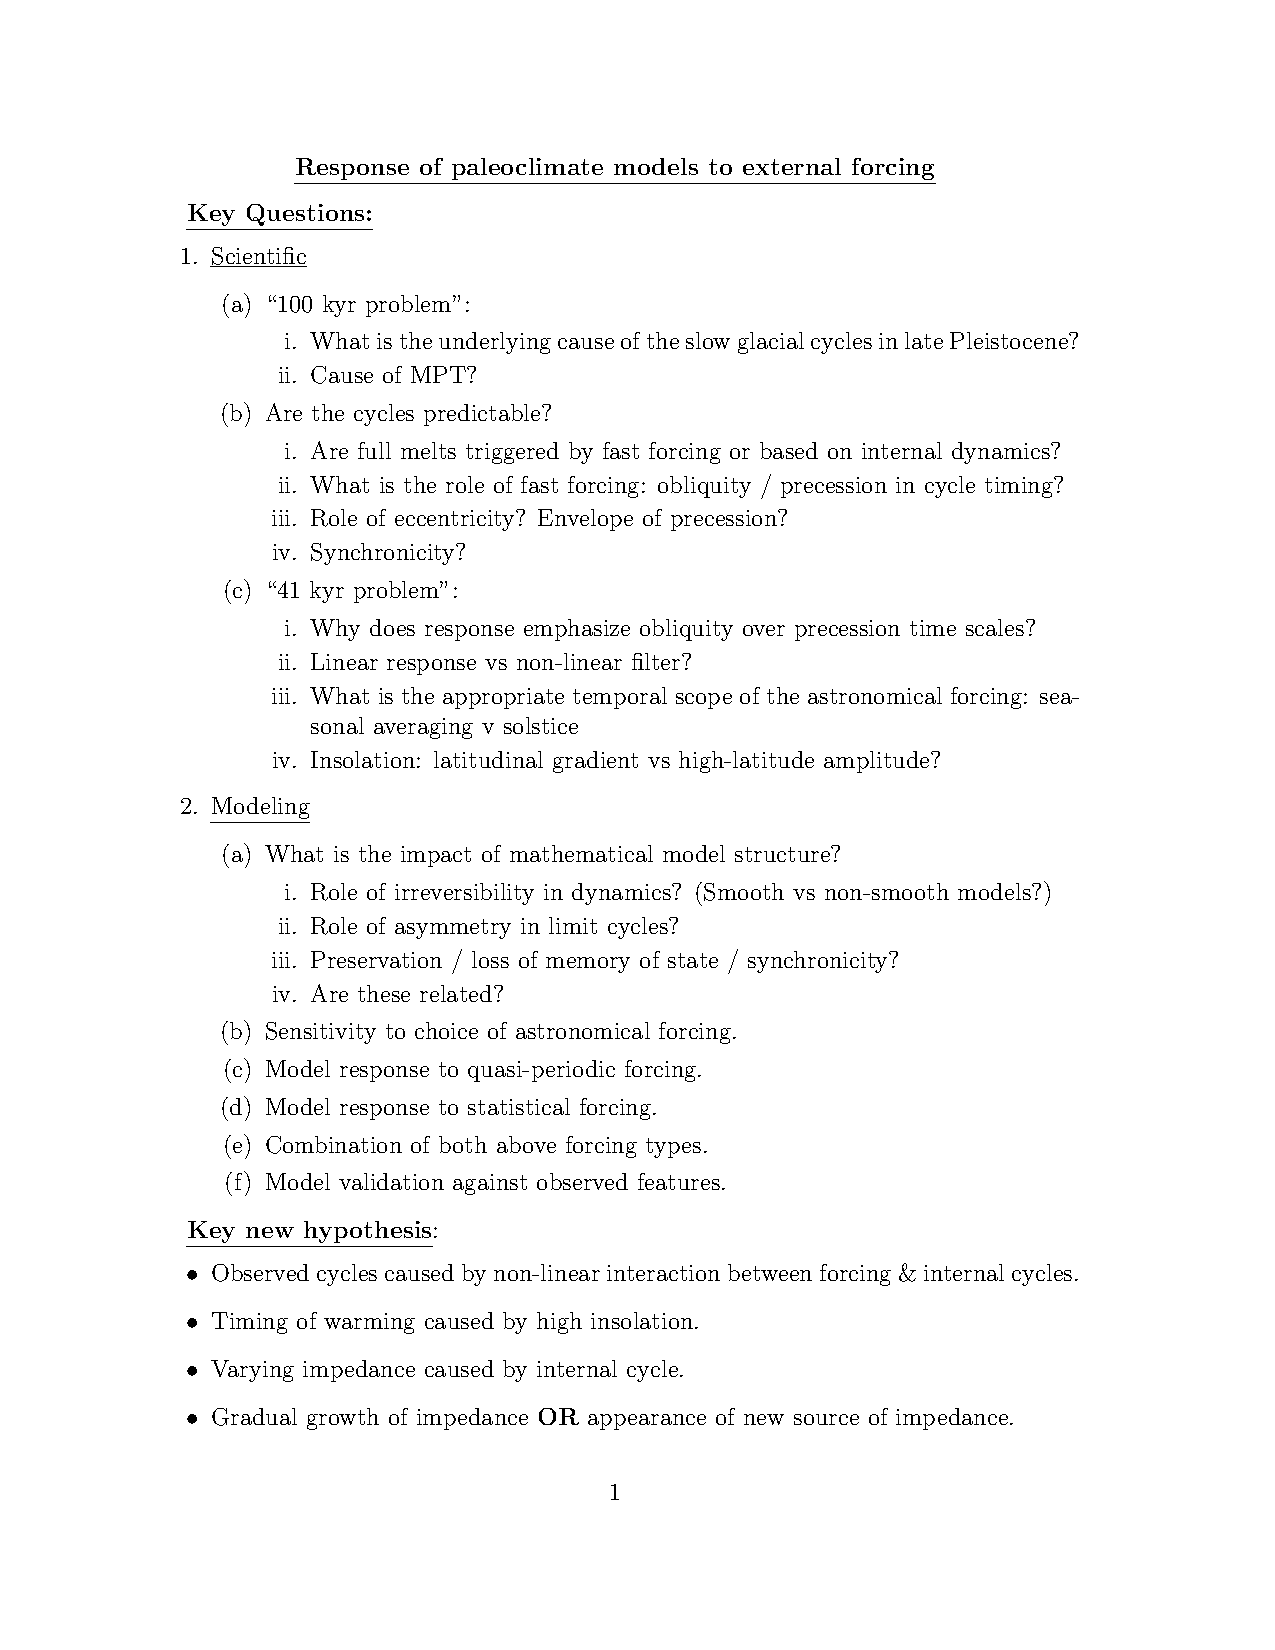
\includepdf[pages=-]{ResearchSummary_SQ19.pdf}
\end{document}
